% v12 --- FIRST CUT of the trimmed opening. Owner's instructions, 2026-09-04:
%   * merge the Introduction (GFL/GFM) and Project Objectives slides into ONE
%     page, and DROP the Scope block;
%   * cut SSSA -- the deck now carries PF and TS only;
%   * then modeling, network, case study, with the equations taken from
%     docs/source/report_ieee14_switch_th_rev2.tex;
%   * PF and TS get BASIC equations only, one page is enough;
%   * the source paper's binary switch command m must appear if the code has one.
%
% WHY A NEW FILE rather than an edit of v11: v11.tex is what the delivered PDF
% was built from and its numbers are cited elsewhere. This is a first cut, so it
% has to be judged next to v11, not on top of it.
%
% PREAMBLE is byte-identical to v11.tex:1-56 (same Helvetica path, same theme,
% same colours, same footline), so the two decks render in the same font and a
% frame can be moved between them without adjustment.
%
% SSSA AND OBJECTIVE 1. Objective 1 in v11 read "Power Flow, SSSA, and
% Time-Domain Simulation". With the SSSA slide cut, naming SSSA in the objective
% would promise a page that no longer exists, so it now names PF and TS only.
% Objective 3 changed for the same reason and NOT because the claim changed: the
% selector table's admissibility does rest on a small-signal screen (the damping
% ratio gate), so the slide says the configurations are screened in advance and
% authenticated at the moment of use, without naming the method the deck no
% longer shows. Putting the SSSA slide back is what would let it be named again.
%
% FRAMES: title, contents, intro+objectives, PF+TS, IBR model, mode command,
% network/case study. Results are NOT in this cut; the contents list matches the
% frames that exist, and the commented sixth row is ready for them.
\documentclass{beamer}
\usepackage{fontspec}
\setsansfont[Path=C:/Users/User/AppData/Local/Microsoft/Windows/Fonts/,UprightFont=Helvetica.ttf,BoldFont=Helvetica-Bold.ttf,ItalicFont=Helvetica-Oblique.ttf,BoldItalicFont=Helvetica-BoldOblique.ttf]{Helvetica.ttf}
\usetheme{Berlin}
\usefonttheme[onlymath]{serif}
\setbeamertemplate{footline}{%
  \leavevmode%
  \hbox{%
  \begin{beamercolorbox}[wd=.88\paperwidth,ht=2.6ex,dp=1.1ex,leftskip=1.2em]{author in head/foot}%
    \ifodd\insertframenumber\relax
      \scriptsize An Automatic Following/Forming Framework for Inverter-Based Resources%
    \else
      \scriptsize Department of Electrical Engineering, School of Engineering, KMITL%
    \fi
  \end{beamercolorbox}%
  \begin{beamercolorbox}[wd=.12\paperwidth,ht=2.6ex,dp=1.1ex,center]{date in head/foot}%
    \scriptsize \insertframenumber/\inserttotalframenumber
  \end{beamercolorbox}}%
}

\usepackage{xcolor}
\usepackage{graphicx}
\usepackage{amsmath,amsfonts,amssymb}
\usepackage{bm}
\setcounter{MaxMatrixCols}{20}
\usepackage{booktabs,array,multicol}
\usepackage{tikz}
\usetikzlibrary{arrows.meta,positioning,shapes}

\definecolor{myblue}{rgb}{0.0,0.0,0.7}
\definecolor{pnavy}{HTML}{0F2A4A}
\definecolor{pblue}{HTML}{1D5288}
\definecolor{pgreen}{HTML}{1E7E34}
\definecolor{pred}{HTML}{A93226}
\definecolor{pyellow}{HTML}{B7950B}
\setbeamercolor{item}{fg=myblue}
\setbeamercolor{block title}{bg=myblue,fg=white}
\setbeamercolor{block body}{bg=blue!7,fg=black}
\setbeamercolor{itemize item}{fg=myblue}
\setbeamertemplate{navigation symbols}{}
\setbeamercolor{frametitle}{bg=myblue!82!black,fg=white}
\setbeamertemplate{section in toc}[sections numbered]
\setbeamertemplate{background}{}
\setbeamertemplate{headline}{}
% Numbered figures and equations, 2026-09-04: every figure and every equation
% must carry a number so it can be pointed at during questions. Beamer's default
% caption template prints no number, hence [numbered]; equation/align number
% themselves once amsmath is loaded.
\setbeamertemplate{caption}[numbered]
\setbeamerfont{caption}{size=\scriptsize}
\setbeamercolor{caption name}{fg=pnavy}

\title{\large\textbf{An Automatic Following/Forming Framework\\for Inverter-Based Resources}}
\author{Phichitchai Jueajan\quad 66010569\\Pakkapol Phdungdan\quad 66010612\\[0.2cm]
Advisor: Dr. Tossaporn Surinkaew\\Co-advisor: Prof. Dr. Issarachai Ngamroo}
\institute{Department of Electrical Engineering, School of Engineering\\
King Mongkut's Institute of Technology Ladkrabang (KMITL)}
\date{}
\titlegraphic{}
\newcommand{\pu}{\,\mathrm{p.u.}}

\begin{document}

% ========================= 1. TITLE ======================================
\begin{frame}[plain]
\centering
\vspace{0.75cm}
\begin{beamercolorbox}[wd=0.86\paperwidth,sep=0.22cm,center]{title}
{\Large\bfseries An Automatic Following/Forming Framework\\for Inverter-Based Resources}
\end{beamercolorbox}
\vspace{0.60cm}
{\fontsize{10.5}{13}\selectfont
Phichitchai Jueajan\quad 66010569\\
Pakkapol Phdungdan\quad 66010612\\[0.20cm]
Advisor: Dr. Tossaporn Surinkaew\\
Co-advisor: Prof. Dr. Issarachai Ngamroo\\[0.45cm]
Department of Electrical Engineering, School of Engineering\\
King Mongkut's Institute of Technology Ladkrabang (KMITL)
}
\end{frame}

% ========================= 2. TABLE OF CONTENTS ==========================
% ABBREVIATION RULE, 2026-09-04: an abbreviation may be used only after it has
% been spelled out once. The contents list is the FIRST place a reader looks, so
% nothing may be abbreviated here -- row 2 spells out both names, and the deck
% introduces PF and TS on the slide that row points to.
%
% Five rows, not v11's six: SSSA is cut, and Introduction/Objectives are now one
% page. The Results row stays commented until those frames exist, so the list
% never promises a section the deck does not contain.
\begin{frame}{Table of Contents}
\centering
\renewcommand{\arraystretch}{1.65}
\begin{tabular}{c@{\hspace{0.35cm}}l}
\colorbox{myblue}{\makebox[0.52cm][c]{\color{white}\Large 1}} & {\Large Introduction and Objectives}\\
\colorbox{myblue}{\makebox[0.52cm][c]{\color{white}\Large 2}} & {\Large Power Flow and Time-Domain Formulation}\\
\colorbox{myblue}{\makebox[0.52cm][c]{\color{white}\Large 3}} & {\Large Converter Modeling}\\
\colorbox{myblue}{\makebox[0.52cm][c]{\color{white}\Large 4}} & {\Large Mode-Switching Command}\\
\colorbox{myblue}{\makebox[0.52cm][c]{\color{white}\Large 5}} & {\Large Network and Case Study}
%\colorbox{myblue}{\makebox[0.52cm][c]{\color{white}\Large 6}} & {\Large Results and Conclusions}
\end{tabular}
\end{frame}

% ============ 3. INTRODUCTION + OBJECTIVES, ONE PAGE =====================
% Owner's correction, 2026-09-04: too much text -- assume the audience knows
% NOTHING. So the physics is told as a three-panel picture and the objectives are
% four short lines. Everything a listener can be told out loud has been taken off
% the slide.
%
% The three panels ARE the whole motivation: (1) the machine holds the angle and
% the converters follow it; (2) the machine leaves and the followers have nothing
% to follow; (3) one converter is promoted and becomes the reference. Panel 3 is
% what the project builds, so it is the one drawn in green.
%
% ABBREVIATIONS: this is their FIRST appearance in the deck, so the line under
% the figure spells both out. Every later slide may then write SG and IBR bare.
\section{Introduction and Objectives}
\begin{frame}{Why a Converter Must Sometimes Lead}
\centering
% GEOMETRY NOTE: the arc label sits at about y=2.1, so the panel title has to
% clear it (y=2.9) and the caption has to clear the box underside at y=1.28
% (caption top-anchored at y=1.05). The first draft put all three at 2.35/1.55/
% 0.85 and every one of them collided in the render. Panel pitch is 4.10 with the
% third caption 3.9 cm wide, so the drawing spans about 11.3 cm before scaling --
% scale 0.94 keeps the third IBR box and its caption inside the text block, which
% the first pass at 1.06 did not.
\begin{figure}
\centering
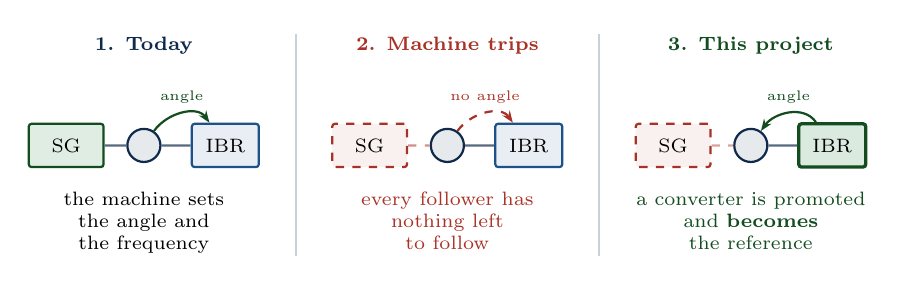
\begin{tikzpicture}[
  font=\scriptsize,
  scale=0.94,
  bus/.style={circle,draw=pnavy,thick,fill=pnavy!10,minimum size=0.42cm,inner sep=0pt},
  mach/.style={draw=pgreen!60!black,thick,fill=pgreen!14,rounded corners=1pt,
               minimum width=0.95cm,minimum height=0.55cm,align=center},
  gone/.style={draw=pred,thick,dashed,fill=pred!7,rounded corners=1pt,
               minimum width=0.95cm,minimum height=0.55cm,align=center},
  flw/.style={draw=pblue,thick,fill=pblue!10,rounded corners=1pt,
              minimum width=0.85cm,minimum height=0.55cm,align=center},
  frm/.style={draw=pgreen!60!black,very thick,fill=pgreen!16,rounded corners=1pt,
              minimum width=0.85cm,minimum height=0.55cm,align=center},
  ln/.style={draw=pnavy!70,thick},
  ok/.style={-{Stealth[length=1.5mm]},draw=pgreen!60!black,thick},
  no/.style={-{Stealth[length=1.5mm]},draw=pred,thick,dashed},
  cpt/.style={align=center,font=\scriptsize,anchor=north},
  ttl/.style={align=center,font=\scriptsize\bfseries}]

% ---------------- panel 1: today ----------------
\node[ttl,pnavy] at (1.35,2.90) {1. Today};
\node[mach] (m1) at (0.30,1.55) {SG};
\node[bus]  (b1) at (1.35,1.55) {};
\node[flw]  (f1) at (2.45,1.55) {IBR};
\draw[ln] (m1) -- (b1); \draw[ln] (b1) -- (f1);
\draw[ok] (b1) to[out=55,in=125] node[midway,above,font=\tiny,pgreen!60!black]
  {angle} (f1);
\node[cpt] at (1.35,1.05) {the machine sets\\the angle and\\the frequency};

\draw[draw=pnavy!22,thick] (3.40,0.05) -- (3.40,3.05);

% ---------------- panel 2: the machine leaves ----------------
\node[ttl,pred] at (5.45,2.90) {2. Machine trips};
\node[gone] (m2) at (4.40,1.55) {SG};
\node[bus]  (b2) at (5.45,1.55) {};
\node[flw]  (f2) at (6.55,1.55) {IBR};
\draw[ln,dashed,draw=pred!55] (m2) -- (b2); \draw[ln] (b2) -- (f2);
\draw[no] (b2) to[out=55,in=125] node[midway,above,font=\tiny,pred]
  {no angle} (f2);
\node[cpt,pred] at (5.45,1.05) {every follower has\\nothing left\\to follow};

\draw[draw=pnavy!22,thick] (7.50,0.05) -- (7.50,3.05);

% ---------------- panel 3: what this project does ----------------
\node[ttl,pgreen!60!black] at (9.55,2.90) {3. This project};
\node[gone] (m3) at (8.50,1.55) {SG};
\node[bus]  (b3) at (9.55,1.55) {};
\node[frm]  (f3) at (10.65,1.55) {IBR};
\draw[ln,dashed,draw=pred!45] (m3) -- (b3); \draw[ln] (b3) -- (f3);
\draw[ok] (f3) to[out=125,in=55] node[midway,above,font=\tiny,pgreen!60!black]
  {angle} (b3);
\node[cpt,pgreen!60!black] at (9.55,1.05)
  {a converter is promoted\\and \textbf{becomes}\\the reference};
\end{tikzpicture}
\caption{A synchronous generator (SG) sets the voltage angle; an inverter-based
resource (IBR) normally follows it.}
\label{fig:why}
\end{figure}

\vspace{-0.10cm}
\hrule
\vspace{0.16cm}
\footnotesize
\begin{columns}[t,onlytextwidth]
\column{0.49\textwidth}
\begin{enumerate}\setlength{\itemsep}{3pt}
  \item One in-house chain: power flow (PF) $\rightarrow$ time-domain simulation
        (TS).
  \item Four converters, one plant, two switchable controllers.
\end{enumerate}
\column{0.49\textwidth}
\begin{enumerate}\setlength{\itemsep}{3pt}\setcounter{enumi}{2}
  \item \textbf{How many} must lead is decided by the network, not fixed by hand.
  \item Verified through trip, fault, and reconnection.
\end{enumerate}
\end{columns}
\end{frame}

% ================ 4. PF AND TS ON ONE PAGE ===============================
% Owner's correction, 2026-09-04: the polar injection sum is a PF detail, not the
% basic statement. PF is now the MISMATCH form -- unknown vector, P and Q
% mismatch driven to zero, one Newton update -- and nothing more. TS carries the
% time variable explicitly, which is the distinction between the two columns:
% PF solves g(x)=0 once, TS solves a t-indexed family of them.
%
% WHERE t ENTERS, so the symbol is not decoration: the network admittance is
% re-stamped at event times, Y_net(t), and each converter's branch selector
% m_i(t) picks which controller block is integrated. Both are read from the
% event schedule, and the solver lands exactly on each event instant.
%
% Sources: KCL/DAE pair -- report_ieee14_switch_th_rev2.tex:227-230 (eq:kcl) and
% 1164-1167 (eq:dae); trapezoidal step -- rev2:1173-1179 (eq:trap); Newton
% tolerance -- rev2:1218.
\section{Power Flow and Time-Domain Formulation}
\begin{frame}{Power Flow and Time-Domain Formulation}
% Numbered equations, per the 2026-09-04 rule. \[ ... \] prints no number, so
% every display here is an equation/align environment instead. PF and TS were
% spelled out on the previous slide and may now be used bare.
%
% LAYOUT, after three collisions in the render:
%   * the Jacobian is its own display -- appended to the Newton update it pushed
%     the number onto the next line and over the following heading;
%   * the TS heading is one short line -- "switched differential-algebraic system"
%     wrapped to two and shifted that whole column down against the equations;
%   * everything is \scriptsize and the closing note is trimmed to two sentences,
%     because at \small the last line fell under the footline.
\begin{columns}[t,onlytextwidth]
\column{0.435\textwidth}
\scriptsize
\textbf{PF --- one steady operating point}
\begin{equation}
\bm x=\begin{bmatrix}\bm\theta\\[1pt]|\bm V|\end{bmatrix}
\end{equation}
\vspace{-0.22cm}
\begin{equation}
\bm g(\bm x)=
\begin{bmatrix}
\bm P^{\mathrm{inj}}-\bm P(\bm x)\\[2pt]
\bm Q^{\mathrm{inj}}-\bm Q(\bm x)
\end{bmatrix}=\bm 0
\end{equation}
\vspace{-0.22cm}
\begin{equation}
\bm x^{(r+1)}=\bm x^{(r)}-\bm J^{-1}\bm g\bigl(\bm x^{(r)}\bigr)
\end{equation}
\vspace{-0.32cm}
\begin{equation}
\bm J=\partial\bm g/\partial\bm x
\end{equation}
\vspace{-0.20cm}

{\tiny No time appears. This point supplies the healthy reference $V_i^{\star}$
per bus and the warm start for the dynamic model.}

\column{0.535\textwidth}
\scriptsize
\textbf{TS --- the same network, stepped in time}
\begin{equation}
\dot{\bm x}=\bm f(\bm x,\bm y,t),\qquad
\bm 0=\bm g(\bm x,\bm y,t)
\end{equation}
\vspace{-0.22cm}
\begin{equation}
\bm X=\begin{bmatrix}\bm x\\[1pt]\bm y\end{bmatrix},\quad
\bm g=\bm Y_{net}(t)\,\bm y-\bm I_{bus}(\bm x,\bm y)
\end{equation}
\vspace{-0.10cm}

Implicit trapezoidal step, $h=t_{n+1}-t_n$:
% Split over two rows: as one display it overran the column by about 15 mm.
\begin{align}
\bm x_{n+1}&=\bm x_n+\tfrac{h}{2}\bigl[\bm f_n+\bm f_{n+1}\bigr]\\
\bm 0&=\bm g(\bm x_{n+1},\bm y_{n+1},t_{n+1})
\end{align}
\vspace{-0.26cm}

{\tiny$\bm f_n=\bm f(\bm x_n,\bm y_n,t_n)$; (7) and (8) are solved together for
$\bm X_{n+1}$ by damped Newton to $\lVert\bm r\rVert_\infty<10^{-8}$. Time enters
through the events: $\bm Y_{net}(t)$ is re-stamped at each one, and $m_i(t)$
picks each converter's controller branch.}
\end{columns}
\end{frame}

% ================ 5. THE IBR MODEL ======================================
% Owner asked for the state vector nested in this order: X_sys = [x_IBR, x_SG],
% then x_IBR, x_SG, x_GFL, x_GFM each expanded.
%
% ONE HONEST NOTE ON ORDER. The slide groups the converters first because that is
% the order asked for. The assembled vector in the code concatenates the SG block
% first (device order SG1, IBR1..IBR4), so the grouping here is a reading order,
% not a claim about index positions -- and no index number is printed, so nothing
% on the slide is falsified by it.
%
% Symbols are the model's own state names: the SG block is the six-coordinate
% machine (+stability/sg_composite_device.m:86) with E_d' frozen, so five of its
% six are integrated; the converter blocks are the GFL and GFM branch names
% (+ibr/gfl_eecon49_full_model.m:178, +ibr/gfm_eecon49_full_model.m:207).
\section{Converter Modeling}
\begin{frame}{One Converter, Two Controller Branches}
% LAYOUT: the frame title is one line (the two-line version pushed the whole body
% down), the figure is 0.80 wide and the three state displays are \scriptsize --
% at \small and 0.92 the third equation fell off the bottom of the frame.
\centering
\begin{figure}
\centering
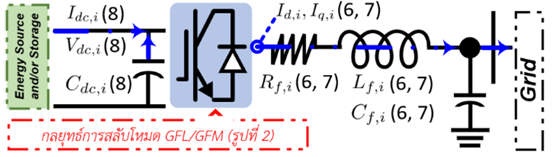
\includegraphics[width=0.80\linewidth]{figures/ibr_plant_eecon49.png}
\caption{One IBR: a shared power stage --- direct-current (DC) link, switching
bridge, alternating-current (AC) filter --- with the GFL/GFM controller branch
selected at run time.}
\label{fig:plant}
\end{figure}

\vspace{-0.02cm}
\scriptsize
\begin{equation}
\bm X_{sys}=\bigl[\,\bm x_{IBR,1}\;\;\bm x_{IBR,2}\;\;\bm x_{IBR,3}\;\;
\bm x_{IBR,4}\;\;\bm x_{SG}\,\bigr]^{\!\top}
\end{equation}
\vspace{-0.30cm}
\begin{equation}
\bm x_{IBR}=\bigl[\underbrace{i_d,\,i_q,\,V_{dc}}_{\text{shared plant}}\;\;
\bm x_{GFL}\;\;\bm x_{GFM}\;\;\underbrace{I_{dc}}_{\text{source}}\bigr],
\qquad
\bm x_{SG}=\bigl[\,\delta,\,\omega,\,E_q',\,E_d',\,E_q'',\,E_d''\,\bigr]
\end{equation}
\vspace{-0.16cm}
\begin{equation}
\bm x_{GFL}=\bigl[\,\theta_{PLL},\,\xi_{PLL},\,\xi_P,\,\xi_Q,\,\xi_{Id},\,\xi_{Iq}\,\bigr],
\qquad
\bm x_{GFM}=\bigl[\,\theta_{VSG},\,\omega_{VSG},\,E,\,\xi_{Vd},\,\xi_{Vq},\,
\xi_{Id},\,\xi_{Iq}\,\bigr]
\end{equation}
\end{frame}

% ================ 6. THE MODE COMMAND ===================================
% Owner's correction, 2026-09-04: (a) the flowchart ran off the slide, and (b) the
% page must describe OUR code, not the source paper.
%
% WHAT OUR CODE ACTUALLY CARRIES -- read from the model and the supervisor, and
% this is where it DIFFERS from the paper's m_i(t):
%
%   1. There is no scalar binary in the state. Each device carries a mode LABEL
%      with three values -- follow, lead, out of service -- plus a separate
%      in-service flag (+ibr/eecon49_dual_mode_model.m:370-394, set at :348-368).
%      A single 0/1 cannot express the third value, so the slide shows the label.
%   2. The right-hand side is a SWITCH, not the paper's m*f_GFM+(1-m)*f_GFL
%      weighted sum: one branch is evaluated and the other block's rows stay zero
%      (dual_f:174-195), and the integrator's active row set changes with the
%      label -- {plant, GFL, source}, {plant, GFM, source}, or empty
%      (active_indices:275-279, sets at :95-96). A weighted sum would evaluate
%      both branches; ours never does.
%   3. The decision is NOT four independent per-converter thresholds. When any
%      following converter's severity crosses, the supervisor asks a
%      pre-authenticated table for the smallest admissible CONFIGURATION -- which
%      converters lead AND which one owns the angle reference -- and commits that
%      row or refuses (ts_simulate_ibr_hybrid.m:852-903). So the command is a
%      table row, not a bit vector, and that is the project's own contribution.
%
% GEOMETRY: beamer's text block is about 10.8 cm wide. The first pass laid five
% boxes plus two outcomes on one row spanning 13 cm and two boxes fell off the
% page. Now four boxes across (right edge at 9.4 cm) with the two outcomes on a
% second row underneath.
\section{Mode-Switching Command}
\begin{frame}{How the Mode Switches}
\centering
\begin{figure}
\centering
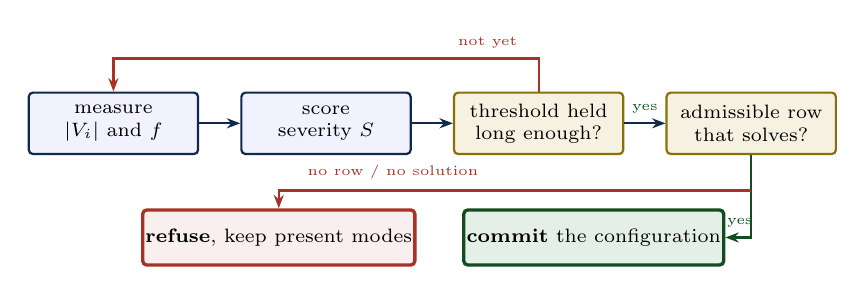
\begin{tikzpicture}[
  font=\scriptsize,
  b/.style={draw=pnavy,thick,fill=blue!5,rounded corners=1.5pt,
            minimum width=2.15cm,minimum height=0.78cm,align=center,inner sep=1pt},
  d/.style={draw=pyellow!75!black,thick,fill=pyellow!12,rounded corners=1.5pt,
            minimum width=2.15cm,minimum height=0.78cm,align=center,inner sep=1pt},
  g/.style={draw=pgreen!60!black,very thick,fill=pgreen!12,rounded corners=1.5pt,
            minimum width=3.10cm,minimum height=0.70cm,align=center,inner sep=1pt},
  r/.style={draw=pred,very thick,fill=pred!8,rounded corners=1.5pt,
            minimum width=3.10cm,minimum height=0.70cm,align=center,inner sep=1pt},
  a/.style={-{Stealth[length=1.7mm]},draw=pnavy,thick},
  ay/.style={-{Stealth[length=1.7mm]},draw=pgreen!60!black,thick},
  an/.style={-{Stealth[length=1.7mm]},draw=pred,thick}]

\node[b] (meas) at (0,0)    {measure\\$|V_i|$ and $f$};
\node[b] (sc)   at (2.70,0) {score\\severity $S$};
\node[d] (dw)   at (5.40,0) {threshold held\\long enough?};
\node[d] (ck)   at (8.10,0) {admissible row\\that solves?};
\draw[a] (meas) -- (sc);
\draw[a] (sc) -- (dw);
\draw[a] (dw) -- node[above,font=\tiny,pgreen!60!black]{yes} (ck);

\node[g] (ok) at (6.10,-1.45) {\textbf{commit} the configuration};
\node[r] (no) at (2.10,-1.45) {\textbf{refuse}, keep present modes};
\draw[ay] (ck.south) |- node[pos=0.72,above,font=\tiny,pgreen!60!black]{yes} (ok.east);
\draw[an] (ck.south) ++(0,-0.45) -| (no.north);
\node[font=\tiny,pred] at (3.55,-0.62) {no row / no solution};
% "not yet" returns to measuring: a dwell that has not elapsed is a wait, not a
% refusal, and drawing it as one would misstate the supervisor.
\draw[an] (dw.north) -- ++(0,0.42) -| node[pos=0.06,above,font=\tiny,pred]{not yet}
  (meas.north);
\end{tikzpicture}
\caption{The decision path: a threshold crossing is a request, and the last box
can refuse it.}
\label{fig:decide}
\end{figure}

\vspace{-0.04cm}
\begin{columns}[t,onlytextwidth]
\column{0.475\textwidth}
\scriptsize
\textbf{What is measured and scored}
% Stacked, not side by side: at \scriptsize in a 0.475-width column the pair on
% one line left no room for the equation number and it wrapped under the fraction.
% Spacing is asymmetric on purpose -- -0.36 closes the gap after a plain line, but
% only -0.16 after a fraction, whose subscripted denominator (Delta f_base) sits
% low enough that -0.36 pulled the next display into its descender.
\vspace{-0.06cm}
\begin{equation}
J_V=\frac{\bigl|\,|V_i|-V_i^{\star}\,\bigr|}{\Delta V_{base}}
\end{equation}
\vspace{-0.30cm}
\begin{equation}
J_f=\frac{|f_{coi}-f_0|}{\Delta f_{base}}
\end{equation}
\vspace{-0.16cm}
% sat[0,1] rather than the spelled-out min/max: at \scriptsize the nested braces
% ran past the column edge and collided with the equation number.
\begin{equation}
S=\operatorname{sat}_{[0,1]}\!\bigl(\tfrac12 J_V+\tfrac12 J_f\bigr)
\end{equation}
\vspace{-0.24cm}

{\tiny Lead at $S\ge0.65$ held $0.10$~s; follow at $S\le0.35$ held $1.00$~s.}

\column{0.505\textwidth}
\scriptsize
\textbf{What the command is, in this framework}
\vspace{-0.06cm}
\begin{equation}
m_i(t)\in\{\text{follow},\;\text{lead},\;\text{out}\}
\end{equation}
\vspace{-0.36cm}
\begin{equation}
\dot{\bm x}_i=\bm f_{GFL},\quad \bm f_{GFM},\quad\text{or }\bm 0
\end{equation}
\vspace{-0.24cm}

{\tiny One branch runs, the other is held --- and the converters are \textbf{not}
switched independently: the whole configuration comes from a table screened in
advance, or is refused.}
\end{columns}
\end{frame}

% ================ 7. NETWORK AND CASE STUDY =============================
% Same figure and the same bus assignment as v11.tex:160-188, which is the
% delivered network drawing. Dispatch numbers are the ones printed on the figure
% itself, so the slide does not restate them and cannot disagree with it.
\section{Network and Case Study}
\begin{frame}{Network and Case Study: IEEE 14-Bus}
\begin{columns}[c,onlytextwidth]
\column{0.225\textwidth}
\scriptsize
\begin{block}{Resources}
\centering
\setlength{\tabcolsep}{3pt}
\begin{tabular}{ll}
\toprule
Unit & Bus \\
\midrule
$\mathrm{SG}_1$ & 1 \\
$\mathrm{IBR}_1$ & 2 \\
$\mathrm{IBR}_2$ & 3 \\
$\mathrm{IBR}_3$ & 6 \\
$\mathrm{IBR}_4$ & 8 \\
\bottomrule
\end{tabular}
\end{block}
\vspace{0.10cm}
{\tiny$\mathrm{SG}_1$ is the slack bus and the only synchronous reference.
$\mathrm{IBR}_1$--$\mathrm{IBR}_4$ are dual-mode converters.}
\column{0.76\textwidth}
\begin{figure}
\centering
\makebox[\linewidth][c]{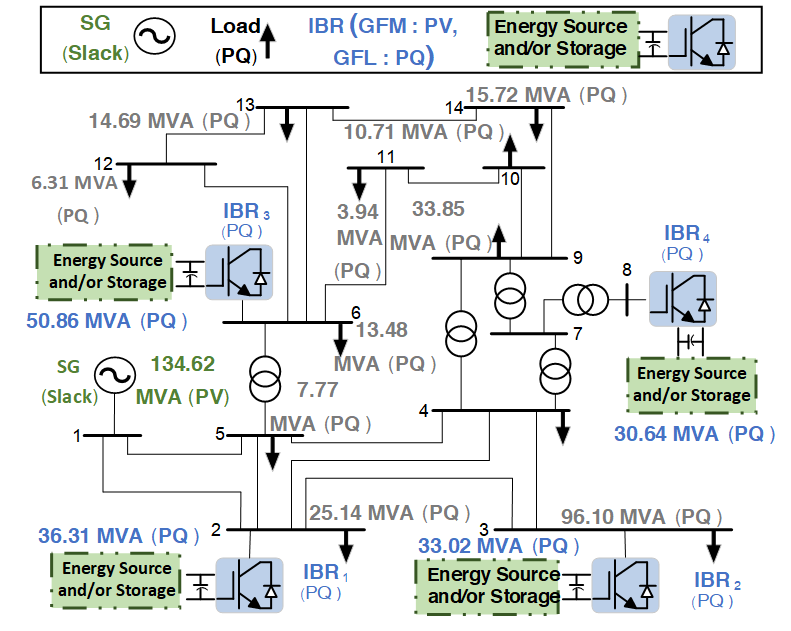
\includegraphics[width=1.00\linewidth]{figures/123313.png}}
% One line: the two-line caption ran under the footline.
\caption{One SG at bus~1 and four dual-mode IBRs at buses 2, 3, 6 and 8.}
\label{fig:network}
\end{figure}
\end{columns}
\end{frame}

\end{document}
